\sectionthree{Partition of integers}
\begin{python0}
from solutions import *; clear() 
\end{python0}

A theory of partition of integers has an extremely long and rich history.
It falls under an area of study called additive number theory.

Let's consider the number 6.
You can write 6 as a sum of positive integers (not including 0) like so:
\begin{align*}
6
&= 6 \\
&= 5 + 1\\
&= 4 + 2 \\
&= 4 + 1 + 1 \\
&= 3 + 3 \\
&= 3 + 2 + 1 \\
&= 3 + 1 + 1 + 1 \\
&= 2 + 2 + 2 \\
&= 2 + 2 + 1 + 1 \\
&= 2 + 1 + 1 + 1 + 1 \\
&= 1 + 1 + 1 + 1 + 1 + 1 
\end{align*}
Each sum on the right (including $6$) is called a \defone{partition} of $6$.
Note that $1 + 5$ is not listed: $1 + 5$ and $5 + 1$ are considered
the same partition.
We say that there are 11 partitions for $6$.
We write $p(n)$\tinysidebar{$p(n)$}\index{p@$p(n)$} for the number of partitions of $n$;
$p(6) = 11$.


\newpage
\begin{ex}
Compute $p(n)$ for $n = 1, ..., 5, 7, 8, 9, 10$.
\end{ex}


\newpage
\begin{ex}
Write a program to list and count partitions.
\end{ex}


\newpage
Note that $p(6)$ is the number of solutions $(a_1, a_2, a_3, a_4, a_5, a_6)$ to
\[
a_1 +  a_2 +  a_3 + a_4 + a_5 + a_6 = 6
\]
where 
\begin{align*}
a_1 &\in \{0, 1, 2, 3, \ldots\} \\
a_2 &\in \{0, 2, 4, 6, \ldots\} \\
a_3 &\in \{0, 3, 6, 9, \ldots\} \\
a_4 &\in \{0, 4, 8, 12, \ldots\} \\
a_5 &\in \{0, 5, 10, 15, \ldots\} \\
a_6 &\in \{0, 6, 12, 18, \ldots\} 
\end{align*}
Right? 
And of course the generation function is
\begin{align*}
f(x) 
&= (1 + x + x^2 + x^3 + \cdots ) \\
& \,\,\,\,\, \times (1 + x^2 + x^4 + x^6 + \cdots ) \\
& \,\,\,\,\, \times (1 + x^3 + x^6 + x^9 + \cdots ) \\
& \,\,\,\,\, \times (1 + x^4 + x^8 + x^{12} + \cdots ) \\
& \,\,\,\,\, \times (1 + x^5 + x^{10} + x^{15} + \cdots ) \\
& \,\,\,\,\, \times (1 + x^6 + x^{12} + x^{18} + \cdots ) 
\end{align*}
(Refer to the previous section on linear forms.)

Of course if you want to consider all the $p(n)$ you need to consider
\begin{align*}
f(x) 
&= (1 + x + x^2 + x^3 + \cdots ) \\
& \,\,\,\,\, \times (1 + x^2 + x^4 + x^6 + \cdots ) \\
& \,\,\,\,\, \times (1 + x^3 + x^6 + x^9 + \cdots ) \\
& \,\,\,\,\, \times (1 + x^4 + x^8 + x^{12} + \cdots ) \\
& \,\,\,\,\, \times (1 + x^5 + x^{10} + x^{15} + \cdots ) \\
& \,\,\,\,\, \times (1 + x^6 + x^{12} + x^{18} + \cdots ) \\
& \,\,\,\,\, \times \cdots \\
&= \frac{1}{1 - x} \cdot \frac{1}{1 - x^2} \cdot \frac{1}{1 - x^3} \cdot \frac{1}{1 - x^4} \cdot \cdots \\
&= \prod_{n=1}^\infty \frac{1}{1 - x^n}
\end{align*}
The $\prod_{n=0}^\infty$ is analogous to the $\sum_{n=0}^\infty$ notation
except that you take the product instead of the sum.
So now I have the generating function for $p(n)$ ($n=0, 1, 2, 3, \ldots$):
\[
\sum_{n=0}^\infty p(n) x^n =  \prod_{n=1}^\infty \frac{1}{1 - x^n}
\]

Besides talking about partitions of $n$,
one can also restrict to certain special partitions.
For instance from the partition of 6
\begin{align*}
6
&= 6 \\
&= 5 + 1\\
&= 4 + 2 \\
&= 4 + 1 + 1 \\
&= 3 + 3 \\
&= 3 + 2 + 1 \\
&= 3 + 1 + 1 + 1 \\
&= 2 + 2 + 2 \\
&= 2 + 2 + 1 + 1 \\
&= 2 + 1 + 1 + 1 + 1 \\
&= 1 + 1 + 1 + 1 + 1 + 1 
\end{align*}
we can look at the \defone{odd partitions} (i.e. partitions of $6$ using only odd terms):
\begin{align*}
6
&= 5 + 1\\
&= 3 + 3 \\
&= 3 + 1 + 1 + 1 \\
&= 1 + 1 + 1 + 1 + 1 + 1 
\end{align*}
We write
\[
p_o(6) = 4\index{p0@$p_0(n)$}
\]

We can also talk about \defone{partitions with distinct terms} of $6$.
In this case we throw away the partition $4 + 1 + 1$ since $1$ is used twice.
The partitions with distinct terms of 6 are
\begin{align*}
6
&= 6 \\
&= 5 + 1\\
&= 4 + 2 \\
&= 3 + 2 + 1 
\end{align*}
We write
\[
p_d(6) = 4\index{pd@$p_d(n)$}
\]


\newpage
\begin{ex}
Write down the generating function for the partition of $n$ where
only even numbers are allowed.
For instance the even partitions of 6 are
\begin{align*}
6
&= 6 \\
&= 4 + 2 \\
&= 2 + 2 + 2 
\end{align*}
Note that there are 3 such partitions.
Verify that the coefficient of $x^6$ in your generating function is 3.
\end{ex}


\newpage
\begin{ex}
Write down the generating function for the partition of $n$ where
every number in a partition can appear at most 3 times.
For instance in the partitions of $6$,
\[
2 + 1 + 1 + 1 + 1 \\
\]
is not allowed since 1 appears 4 times.
For instance the even partitions of 6 are
\begin{align*}
6
&= 6 \\
&= 5 + 1\\
&= 4 + 2 \\
&= 4 + 1 + 1 \\
&= 3 + 3 \\
&= 3 + 2 + 1 \\
&= 3 + 1 + 1 + 1 \\
&= 2 + 2 + 2 \\
&= 2 + 2 + 1 + 1 \\
\end{align*}
Note that there are 9 such partitions.
Verify that the coefficient of $x^6$ in your generating function is 9.
\end{ex}


\newpage
\begin{ex}
Check that $p_o(n) = p_d(n)$ for $n = 1, ... 5$.
\end{ex}


\newpage
We will show that $p_d(n) = p_o(n)$ for \textit{all} $n$.
In fact we'll show that their generating functions are the same
\[
\sum_{n=0}^\infty p_d(n) x^n = 
\sum_{n=0}^\infty p_o(n) x^n 
\]
thereby proving all the equalities in one step.
To do that we'll need to write down the generating functions for $p_d(n)$
and $p_o(n)$.

The generating function for $p_d(n)$ ($n=0,1,...$) is
\[
\sum_{n=0}^\infty p_d(n) x^n
= (1 + x) (1 + x^2) (1 + x^3) \cdots
\]

The generating function for $p_o(n)$ ($n=0,1,...$) is
\begin{align*}
\sum_{n=0}^\infty p_o(n) x^n 
&= (1 + x + x^2 + x^3 + \cdots ) \\
& \,\,\,\,\, \times (1 + x^3 + x^6 + x^9 + \cdots ) \\
& \,\,\,\,\, \times (1 + x^5 + x^{10} + x^{15} + \cdots ) \\
& \,\,\,\,\, \times \cdots \\
&= \frac{1}{1 - x} \cdot \frac{1}{1 - x^3} \cdot\frac{1}{1 - x^5} \cdots 
\end{align*}
We want to show that this is $(1 + x) (1 + x^2) (1 + x^3) \cdots$.
Hmmm ... let's just introduce the factors of this function into $\sum_{n=0}^\infty p_o(n)x^n$.
Let me push $1+x$ into the function like this:
\begin{align*}
\sum_{n=0}^\infty p_o(n) x^n 
&= \frac{1+x}{1+x} \cdot \frac{1}{1 - x} \cdot \frac{1}{1 - x^3} \cdot\frac{1}{1 - x^5} \cdots 
\end{align*}
Now this is
\begin{align*}
\sum_{n=0}^\infty p_o(n) x^n 
&= (1+x) \cdot \frac{1}{(1+x)(1-x)} \cdot \frac{1}{1 - x^3} \cdot\frac{1}{1 - x^5} \cdots \\ 
&= (1+x) \cdot \frac{1}{1 - x^2} \cdot \frac{1}{1 - x^3} \cdot\frac{1}{1 - x^5} \cdots 
\end{align*}
Now what if we do the same by insert $(1+x^2)/(1+x^2)$?
\begin{align*}
\sum_{n=0}^\infty p_o(n) x^n 
&= (1+x) \frac{1+x^2}{1+x^2}\cdot \frac{1}{1 - x^2} \cdot \frac{1}{1 - x^3} \cdot\frac{1}{1 - x^5} \cdots 
\end{align*}
Whoa! It becomes:
\begin{align*}
\sum_{n=0}^\infty p_o(n) x^n 
&= (1+x)(1+x^2) \frac{1}{(1+x^2)(1 - x^2)} \cdot \frac{1}{1 - x^3} \cdot\frac{1}{1 - x^5} \cdots \\
&= (1+x)(1+x^2) \cdot \frac{1}{1 - x^4} \cdot \frac{1}{1 - x^3} \cdot\frac{1}{1 - x^5} \cdots 
\end{align*}
and putting $1/(1-x^4)$ into the right place:
\begin{align*}
\sum_{n=0}^\infty p_o(n) x^n 
&= (1+x)(1+x^2) \frac{1}{(1+x^2)(1 - x^2)} \cdot \frac{1}{1 - x^3} \cdot\frac{1}{1 - x^5} \cdots \\
&= (1+x)(1+x^2) \cdot  \frac{1}{1 - x^3} \cdot \frac{1}{1 - x^4} \cdot \frac{1}{1 - x^5} \cdots 
\end{align*}
It should be clear now that the next step gives us
\begin{align*}
\sum_{n=0}^\infty p_o(n) x^n 
&= (1+x)(1+x^2)(1+x^3) \cdot  \frac{1}{1 - x^6} \cdot \frac{1}{1 - x^4} \cdot \frac{1}{1 - x^5} \cdots  \\
&= (1+x)(1+x^2)(1+x^3) \cdot   \frac{1}{1 - x^4} \cdot \frac{1}{1 - x^5} \cdot \frac{1}{1 - x^6} \cdots 
\end{align*}
And then
\begin{align*}
\sum_{n=0}^\infty p_o(n) x^n 
&= (1+x)(1+x^2)(1+x^3)(1+x^4) \cdot \frac{1}{1 - x^8} \cdot \frac{1}{1 - x^5} \cdot \frac{1}{1 - x^6} \cdots \\
&= (1+x)(1+x^2)(1+x^3)(1+x^4) \cdot \frac{1}{1 - x^5} \cdot 
\frac{1}{1 - x^6} \cdot \frac{1}{1 - x^7} \cdot \frac{1}{1 - x^8} \cdots \\
&= \ldots \\
\end{align*}
You see that the power series is the same as $\sum_{n=0}^\infty p_d(n) x^n$.

In the study of combinatorics and discrete math, 
there are many \lq\lq diagram'' techniques.
The \defone{Ferrers diagram} is a diagram for finding new partitions.
Here's a partition of 7:
\[
4 + 2 + 1
\]
The Ferrers diagram of this partition is
\begin{verbatim}
    * * * *
    * * 
    *
\end{verbatim}
Now if you reflect this diagram about the diagonal
that runs from the top left corner
to the bottom right corner of the diagram 
you get this:
\begin{verbatim}
    * * * 
    * * 
    *
    *
\end{verbatim}
(i.e. make each row of the diagram a column).
You get a new partition
\[
3 + 2 + 1 + 1
\]
Of course this is a partition of 7 since the number of dots
is the same.
You will of course get a new partition if the diagram 
is not symmetric about the mirror line.
For instance the partition
\[
4 + 2 + 1 + 1
\]
of 8 has the Ferrers diagram
\begin{verbatim}
    * * * *
    * *
    *
    *
\end{verbatim}
which when reflected also gives
\begin{verbatim}
    * * * *
    * *
    *
    *
\end{verbatim}
which gives the same partition.


\newpage
\begin{ex}
Consider all the partitions of $6$.
Pair up two partitions if they are obtained from each other
as reflection of their Ferrers diagram.
How many pairs to you get?
How many remaining partitions have symmetric Ferrers diagram?
\end{ex}


\newpage
\begin{ex}
For $n=1, ..., 8$, how many partitions of $n$ have
symmetric Ferrers diagram?
Are there $n$'s without partitions with symmetric Ferrers diagram?
\end{ex}


\newpage
\begin{ex}
Show that if $n = 1 + 2m$, then $n$ must have (at least) one partition
with a symmetric Ferrers diagram.
Write down a partition that is symmetric (i.e. have a symmetric
Ferrers diagram.)
\end{ex}

%
%    *****
%    *
%    *
%    *
%    *
%


\newpage
\begin{ex}
Show that if $n = 2 + 2m$,
then $n$ has at least $1 + \lfloor \frac{m-1}{2} \rfloor$
symmetric partitions. 
Describe the symmetric partitions.
Test it with $n = 2 + 10$ and $n = 2 + 12$.
\end{ex}

% 2 of the 5 x's on both arms can be moved:
%
%    **xxxxx    
%    *o         
%    x          
%    x          
%    x          
%    x          
%    x          
%
%    **xxxx    
%    *ox         
%    xx          
%    x          
%    x          
%    x                  
%
%    **xxx    
%    *oxx         
%    xx          
%    xx          
%    x


\newpage
\begin{ex}
Let an integer $n$ have at least $k$ partitions
made up of $m$ parts where each part is at $> m$.
Is it true that $p(n) \geq 2k$?
\end{ex}


\newpage
\begin{ex}
Here's another method for creating new partitions.
First consider this Ferrers diagram:
\begin{verbatim}
    * * * *
    * * 
    *
\end{verbatim}
This gives a partition of $4 + 2 + 1$, i.e. a partition of $7$.
First ignore the leftmost column:
\begin{verbatim}
    *     * * *
    *     * 
    *
\end{verbatim}
You can the partition 
\begin{verbatim}
          * * *
          * 
\end{verbatim}
i.e. $3 + 1$.
Perform a reflection on it to get
\begin{verbatim}
          * *
          *
          * 
\end{verbatim}
and join it with the original leftmost column 
\begin{verbatim}
    *     * *
    *  <- *   
    *     *
\end{verbatim}
to get this:
\begin{verbatim}
    * * *
    * *   
    * *
\end{verbatim}
i.e. you get $3 + 2 + 2$.
Study this new technique.
\end{ex}

\newpage
\subsection*{Solutions}

\newpage
\section*{Solutions}
Solution to Exercise \ref{ex:dfa0}\labeltext{}{sol:dfa0}.

\tinysidebar{\debug{exercises/{dfa0/answer.tex}}}

    Solution not provided.
    

\newpage

Solution to Exercise \ref{ex:dfa1}\labeltext{}{sol:dfa1}.

\tinysidebar{\debug{exercises/{dfa1/answer.tex}}}
  The ID computation is
  \begin{align*}
    (q_0, aba)
    &\vdash (\delta(q_0, a), ba) = (q_0, ba) \\ 
    &\vdash (\delta(q_0, b), a) = (q_1, a) \\
    &\vdash (\delta(q_1, a), \ep) = (q_0, \ep)
  \end{align*}
  $q_0$ is not an accept state. Therefore $aba$ is not accepted.


\newpage

Solution to Exercise \ref{ex:dfa4}\labeltext{}{sol:dfa4}.

\tinysidebar{\debug{exercises/{dfa4/answer.tex}}}

    Solution not provided.
    

\newpage

Solution to Exercise \ref{ex:dfa5}\labeltext{}{sol:dfa5}.

\tinysidebar{\debug{exercises/{dfa5/answer.tex}}}

    Solution not provided.
    

\newpage

Solution to Exercise \ref{ex:implementing-a-single-dfa0}\labeltext{}{sol:implementing-a-single-dfa0}.

\tinysidebar{\debug{exercises/{implementing-a-single-dfa0/answer.tex}}}

    Solution not provided.
    

\newpage

Solution to Exercise \ref{ex:nfastatediag0}\labeltext{}{sol:nfastatediag0}.

\tinysidebar{\debug{exercises/{nfastatediag0/answer.tex}}}

    Solution not provided.
    

\newpage

Solution to Exercise \ref{ex:nfastatediag1}\labeltext{}{sol:nfastatediag1}.

\tinysidebar{\debug{exercises/{nfastatediag1/answer.tex}}}

    Solution not provided.
    

\newpage

Solution to Exercise \ref{ex:nfastatediag2}\labeltext{}{sol:nfastatediag2}.

\tinysidebar{\debug{exercises/{nfastatediag2/answer.tex}}}

    Solution not provided.
    

\newpage

Solution to Exercise \ref{ex:nfastatediag3}\labeltext{}{sol:nfastatediag3}.

\tinysidebar{\debug{exercises/{nfastatediag3/answer.tex}}}

    Solution not provided.
    

\newpage

Solution to Exercise \ref{ex:nfastatediag4}\labeltext{}{sol:nfastatediag4}.

\tinysidebar{\debug{exercises/{nfastatediag4/answer.tex}}}

    Solution not provided.
    

\newpage

Solution to Exercise \ref{ex:nfastatediag5}\labeltext{}{sol:nfastatediag5}.

\tinysidebar{\debug{exercises/{nfastatediag5/answer.tex}}}

    Solution not provided.
    

\newpage

Solution to Exercise \ref{ex:nfastatediag6}\labeltext{}{sol:nfastatediag6}.

\tinysidebar{\debug{exercises/{nfastatediag6/answer.tex}}}

    Solution not provided.
    

\newpage

Solution to Exercise \ref{ex:nfastatediag7}\labeltext{}{sol:nfastatediag7}.

\tinysidebar{\debug{exercises/{nfastatediag7/answer.tex}}}

    Solution not provided.
    

\newpage

Solution to Exercise \ref{ex:nfastatediag8}\labeltext{}{sol:nfastatediag8}.

\tinysidebar{\debug{exercises/{nfastatediag8/answer.tex}}}

    Solution not provided.
    

\newpage

Solution to Exercise \ref{ex:nfastatediag9}\labeltext{}{sol:nfastatediag9}.

\tinysidebar{\debug{exercises/{nfastatediag9/answer.tex}}}

    Solution not provided.
    

\newpage

Solution to Exercise \ref{ex:nfastatediag10}\labeltext{}{sol:nfastatediag10}.

\tinysidebar{\debug{exercises/{nfastatediag10/answer.tex}}}

    Solution not provided.
    

\newpage

Solution to Exercise \ref{ex:nfastatediag11}\labeltext{}{sol:nfastatediag11}.

\tinysidebar{\debug{exercises/{nfastatediag11/answer.tex}}}

    Solution not provided.
    

\newpage

Solution to Exercise \ref{ex:nfastatediag12}\labeltext{}{sol:nfastatediag12}.

\tinysidebar{\debug{exercises/{nfastatediag12/answer.tex}}}

    Solution not provided.
    

\newpage

Solution to Exercise \ref{ex:nfastatediag13}\labeltext{}{sol:nfastatediag13}.

\tinysidebar{\debug{exercises/{nfastatediag13/answer.tex}}}

    Solution not provided.
    

\newpage

Solution to Exercise \ref{ex:nfa0}\labeltext{}{sol:nfa0}.

\tinysidebar{\debug{exercises/{nfa0/answer.tex}}}
The formal definition of this NFA is $(\Sigma, Q, q_0, \delta, F)$ where
\begin{tightlist}
\li $\Sigma = \{a,b\}$
\li $Q = \{q_0\}$
\li $\delta$ is the function
\[
\delta : Q \times \Sigma_\epsilon \rightarrow P(Q)
\]
given by
\begin{align*}
  \delta(q_0, \epsilon) &= \{\} \\
  \delta(q_0, a) &= \{\} \\
  \delta(q_0, b) &= \{\} 
\end{align*}
\end{tightlist}


\newpage

Solution to Exercise \ref{ex:nfa1}\labeltext{}{sol:nfa1}.

\tinysidebar{\debug{exercises/{nfa1/answer.tex}}}

    Solution not provided.
    

\newpage

Solution to Exercise \ref{ex:nfa2}\labeltext{}{sol:nfa2}.

\tinysidebar{\debug{exercises/{nfa2/answer.tex}}}

    Solution not provided.
    

\newpage

Solution to Exercise \ref{ex:nfa3}\labeltext{}{sol:nfa3}.

\tinysidebar{\debug{exercises/{nfa3/answer.tex}}}

    Solution not provided.
    

\newpage

Solution to Exercise \ref{ex:nfa4}\labeltext{}{sol:nfa4}.

\tinysidebar{\debug{exercises/{nfa4/answer.tex}}}

    Solution not provided.
    

\newpage

Solution to Exercise \ref{ex:nfa5}\labeltext{}{sol:nfa5}.

\tinysidebar{\debug{exercises/{nfa5/answer.tex}}}

    Solution not provided.
    

\newpage

Solution to Exercise \ref{ex:dfa-as-powerful-as-nfa0}\labeltext{}{sol:dfa-as-powerful-as-nfa0}.

\tinysidebar{\debug{exercises/{dfa-as-powerful-as-nfa0/answer.tex}}}
Here's the solution.
Let $\delta$ denote the transition function of $N$.
Note that 
\begin{align*}
  \delta(q_0, \epsilon) = \{\} \\
  \delta(q_0, a) = \{\} \\
  \delta(q_0, b) = \{\} 
\end{align*}
First of all the states are labeled as all the subsets of $\{q_0\}$.


\begin{center}
\begin{tikzpicture}[>=triangle 60,shorten >=0.5pt,node distance=2cm,auto,initial text=, double distance=2pt]
\node[state] (A) at (  0,  0) {$\{q_0\}$};
\node[state] (B) at (  3,  0) {$\{\}$};

\path[->]

;
\end{tikzpicture}
\end{center}
    


The start state is the $\epsilon$-closure of $\{q_0\}$.
However in $N$, there are no $\epsilon$--transitions out of 
$q_0$.
So the $\epsilon$-closure of $\{q_0\}$ is in fact $\{q_0\}$, i.e.
$\overline{\{q_0\}} = \{q_0\}$
The $\DFA$ is now this:


\begin{longtable}{|r||r|r|r|r|r|}
\hline 
         & $w_1$ & $w_2$ & $w_3$ & $w_4$ & $\ldots$ \\ \hline \hline 
$M_1$    &       &       &       &       &          \\ \hline 
$M_2$    &       &       &       &       &          \\ \hline 
$M_3$    &       &       &       &       &          \\ \hline 
$M_4$    &       &       &       &       &          \\ \hline 
$\ldots$ &       &       &       &       &          \\ \hline 
\end{longtable}
        


Now I will compute the $a$--transition of the state $\{q_0\}$.
Let $\delta^\DFA$ denote the transition function of the $\DFA$
that we're building.
Then
\begin{align*}
\delta( \{q_0, a\} ) 
&= \overline{ \bigcup_{q \in \{q_0\}} \delta(q, a)} \\
&= \overline{ \delta(q_0, a) } \\
&= \overline{ \emptyset } \\
&= \emptyset
\end{align*}
The (incomplete) $\DFA$ now looks like this:


\begin{longtable}{|r||r|r|r|r|r|}
\hline 
         & $w_1$ & $w_2$ & $w_3$ & $w_4$ & $\ldots$ \\ \hline \hline 
$M_1$    & 0     & 0     & 1     & 0     & ...      \\ \hline 
$M_2$    & 1     & 0     & 1     & 1     & ...      \\ \hline 
$M_3$    & 0     & 1     & 1     & 1     & ...      \\ \hline 
$M_4$    & 1     & 0     & 1     & 1     & ...      \\ \hline 
$\ldots$ &       &       &       &       &          \\ \hline 
\end{longtable}
        


Using the same reasoning we have

\begin{center}
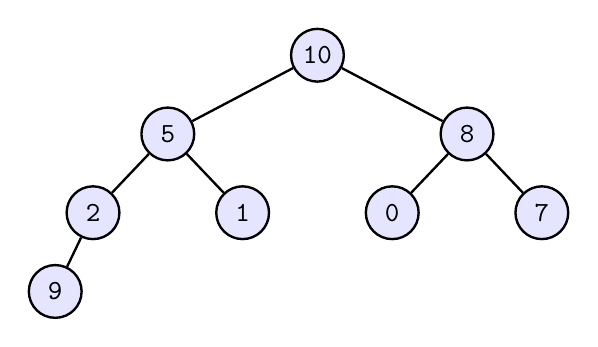
\begin{tikzpicture}

\fill[blue!10] (0.0, 0.0) circle (0.35);
\node [line width=0.03cm,black,minimum size=0.6699999999999999cm,draw,circle] at (0.0,0.0)(10){};\draw (0.0, 0.0) node[color=black] {\texttt{10}};
\fill[blue!10] (-1.9, -1.0) circle (0.35);
\node [line width=0.03cm,black,minimum size=0.6699999999999999cm,draw,circle] at (-1.9,-1.0)(5){};\draw (-1.9, -1.0) node[color=black] {\texttt{5}};
\fill[blue!10] (1.9, -1.0) circle (0.35);
\node [line width=0.03cm,black,minimum size=0.6699999999999999cm,draw,circle] at (1.9,-1.0)(8){};\draw (1.9, -1.0) node[color=black] {\texttt{8}};
\fill[blue!10] (-2.85, -2.0) circle (0.35);
\node [line width=0.03cm,black,minimum size=0.6699999999999999cm,draw,circle] at (-2.85,-2.0)(2){};\draw (-2.85, -2.0) node[color=black] {\texttt{2}};
\fill[blue!10] (-0.95, -2.0) circle (0.35);
\node [line width=0.03cm,black,minimum size=0.6699999999999999cm,draw,circle] at (-0.95,-2.0)(1){};\draw (-0.95, -2.0) node[color=black] {\texttt{1}};
\fill[blue!10] (0.95, -2.0) circle (0.35);
\node [line width=0.03cm,black,minimum size=0.6699999999999999cm,draw,circle] at (0.95,-2.0)(0){};\draw (0.95, -2.0) node[color=black] {\texttt{0}};
\fill[blue!10] (2.85, -2.0) circle (0.35);
\node [line width=0.03cm,black,minimum size=0.6699999999999999cm,draw,circle] at (2.85,-2.0)(7){};\draw (2.85, -2.0) node[color=black] {\texttt{7}};
\fill[blue!10] (-3.33, -3.0) circle (0.35);
\node [line width=0.03cm,black,minimum size=0.6699999999999999cm,draw,circle] at (-3.33,-3.0)(9){};\draw (-3.33, -3.0) node[color=black] {\texttt{9}};\draw[line width=0.03cm,black] (10) to  (5);
\draw[line width=0.03cm,black] (10) to  (8);
\draw[line width=0.03cm,black] (5) to  (2);
\draw[line width=0.03cm,black] (5) to  (1);
\draw[line width=0.03cm,black] (8) to  (0);
\draw[line width=0.03cm,black] (8) to  (7);
\draw[line width=0.03cm,black] (2) to  (9);
\end{tikzpicture}

\end{center}



It's easy to see that in the DFA, the $a$--
and $b$--transitions from the state $\{\}$ goes back to itself.
Therefore the completed DFA is this:


\begin{center}
\begin{tikzpicture}[>=triangle 60,shorten >=0.5pt,node distance=2cm,auto,initial text=, double distance=2pt]
\node[state,initial] (A) at (  0,  0) {$\{q_0\}$};
\node[state] (B) at (  3,  0) {$\{\}$};

\path[->]
(A) edge [bend left=0,pos=0.5,above] node {$a,b$} (B)
(B) edge [loop above] node {$a,b$} ()

;
\end{tikzpicture}
\end{center}
    



\newpage

Solution to Exercise \ref{ex:dfa-as-powerful-as-nfa1}\labeltext{}{sol:dfa-as-powerful-as-nfa1}.

\tinysidebar{\debug{exercises/{dfa-as-powerful-as-nfa1/answer.tex}}}

    Solution not provided.
    

\newpage

Solution to Exercise \ref{ex:dfa-as-powerful-as-nfa2}\labeltext{}{sol:dfa-as-powerful-as-nfa2}.

\tinysidebar{\debug{exercises/{dfa-as-powerful-as-nfa2/answer.tex}}}

    Solution not provided.
    

\newpage

Solution to Exercise \ref{ex:dfa-as-powerful-as-nfa3}\labeltext{}{sol:dfa-as-powerful-as-nfa3}.

\tinysidebar{\debug{exercises/{dfa-as-powerful-as-nfa3/answer.tex}}}

    Solution not provided.
    

\newpage

Solution to Exercise \ref{ex:dfa-as-powerful-as-nfa4}\labeltext{}{sol:dfa-as-powerful-as-nfa4}.

\tinysidebar{\debug{exercises/{dfa-as-powerful-as-nfa4/answer.tex}}}

    Solution not provided.
    

\newpage

Solution to Exercise \ref{ex:closure0}\labeltext{}{sol:closure0}.

\tinysidebar{\debug{exercises/{closure0/answer.tex}}}

    Solution not provided.
    

\newpage

Solution to Exercise \ref{ex:closure1}\labeltext{}{sol:closure1}.

\tinysidebar{\debug{exercises/{closure1/answer.tex}}}

    Solution not provided.
    

\newpage

Solution to Exercise \ref{ex:closure2}\labeltext{}{sol:closure2}.

\tinysidebar{\debug{exercises/{closure2/answer.tex}}}

    Solution not provided.
    

\newpage

Solution to Exercise \ref{ex:closure3}\labeltext{}{sol:closure3}.

\tinysidebar{\debug{exercises/{closure3/answer.tex}}}

    Solution not provided.
    

\newpage

Solution to Exercise \ref{ex:closure4}\labeltext{}{sol:closure4}.

\tinysidebar{\debug{exercises/{closure4/answer.tex}}}

    Solution not provided.
    

\newpage

Solution to Exercise \ref{ex:closure5}\labeltext{}{sol:closure5}.

\tinysidebar{\debug{exercises/{closure5/answer.tex}}}

    Solution not provided.
    

\newpage

Solution to Exercise \ref{ex:closure6}\labeltext{}{sol:closure6}.

\tinysidebar{\debug{exercises/{closure6/answer.tex}}}

    Solution not provided.
    

\newpage

Solution to Exercise \ref{ex:closure7}\labeltext{}{sol:closure7}.

\tinysidebar{\debug{exercises/{closure7/answer.tex}}}

    Solution not provided.
    

\newpage

Solution to Exercise \ref{ex:closure8}\labeltext{}{sol:closure8}.

\tinysidebar{\debug{exercises/{closure8/answer.tex}}}

    Solution not provided.
    

\newpage

Solution to Exercise \ref{ex:closure9}\labeltext{}{sol:closure9}.

\tinysidebar{\debug{exercises/{closure9/answer.tex}}}

    Solution not provided.
    

\newpage

Solution to Exercise \ref{ex:closure10}\labeltext{}{sol:closure10}.

\tinysidebar{\debug{exercises/{closure10/answer.tex}}}

    Solution not provided.
    

\newpage

Solution to Exercise \ref{ex:closure11}\labeltext{}{sol:closure11}.

\tinysidebar{\debug{exercises/{closure11/answer.tex}}}

    Solution not provided.
    

\newpage

Solution to Exercise \ref{ex:closure12}\labeltext{}{sol:closure12}.

\tinysidebar{\debug{exercises/{closure12/answer.tex}}}

    Solution not provided.
    


